\documentclass[12pt]{article}
\usepackage[reqno]{amsmath}
\usepackage{amsfonts}
\usepackage{mathtools}
\usepackage{amssymb}
\usepackage{amsthm}
%\usepackage{multicol}
\usepackage[a4paper, margin=1in]{geometry}
\usepackage{indentfirst}
\usepackage{bm}
\usepackage{wrapfig}
\usepackage{enumitem}
\usepackage{mwe}
\usepackage{hyperref}
\hypersetup{
    colorlinks=true,
    linkcolor=blue,      
    urlcolor=cyan,
}
\renewcommand{\thesection}{\Roman{section}}
\setlength{\parindent}{4em}


\begin{document}
\begin{center}
\par\noindent\rule{\textwidth}{0.6pt}\\[0.3cm]
\textbf{\LARGE{Assignment 3}}\\[0.3cm]
\Large{BT1010 : Introduction to Life Sciences}\\[0.1cm]
\large{April 7, 2021}\\[0cm]
\par\noindent\rule{\textwidth}{0.6pt}
\end{center}
%\begin{multicols}{2}
\noindent
\hspace{0.4cm}Name : Taha Adeel Mohammed
\par \noindent
\hspace{0.4cm}Roll No. : CS20BTECH11052
\section*{Question}
In the picture A and B (see below) pedigree of a trait controlled by either dominant or recessive gene action is shown. Explain which pedigree represents dominant and which one represent recessive gene and why?
\begin{figure}[h]
\centering
\begin{minipage}{.5\textwidth}
  \centering
  \captionof{\textbf{A}}
  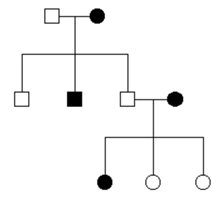
\includegraphics{Figures/Picture1_original.png}
  
\end{minipage}%
\begin{minipage}{.5\textwidth}
  \captionof{\textbf{B}}
  \centering
  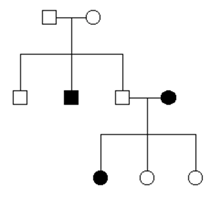
\includegraphics{Figures/Picture2_original.png}

\end{minipage}
\end{figure}

\section*{Answer}
\noindent In the solution, the alleles are represented as \texttt{A} and \texttt{a}, and the trees have been numbered for easy reference while explaining.\\
\begin{wrapfigure}{r}{0.4\textwidth}
\vspace{-6mm}
    \centering
    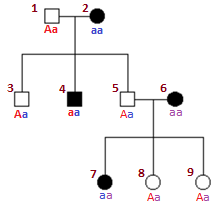
\includegraphics[width=.8\linewidth]{Figures/Picture1_recessive.png}
    \caption{Disorder is recessive}
\end{wrapfigure}
\noindent\textbf{A)  \,\,(\texttt{i})} Let the disorder allele be \textbf{recessive}. Then $2,4,6$ and $7$ have to be \texttt{aa}. As $4$ is \texttt{aa}, it has to get one \texttt{a} from $1$, and $1$ shouldn't have the disorder. Therefore $1$ has to be \texttt{Aa}. As $2$ is \texttt{aa}, $3$ and $5$ must be \texttt{Aa}. Similarly, as $6$ is \texttt{aa}, $8$ and $9$ must be \texttt{Aa}. Hence we do not reach any inconsistency if the disorder is recessive.
Therefore the disorder can be recessive.
\\\\\\\\\\\\\

\begin{wrapfigure}{r}{0.4\textwidth}
    \centering
    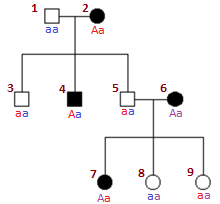
\includegraphics[width=.8\linewidth]{Figures/Picture1_dominant.png}
    \caption{Disorder is dominant}
\end{wrapfigure}
\par\noindent\textbf{\;\;\;\;\;\,\,(\texttt{ii})} Let the disorder allele be \textbf{dominant}. Then $1,3,5,8$ and $9$ have to be \texttt{aa}. As $3 , 5$, and $8 , 9$ are \texttt{aa}, they have to get one \texttt{a} from $2$ and $6$ respectively. Therefore $2$ and $6$ are \texttt{Aa}. As $1$ and $5$ are \texttt{aa}, $4$ and $7$ must respectively be \texttt{Aa}. Again, we do not reach any inconsistency if the disorder is dominant.
\begin{align*}
    \textbf{Therefore the disorder can be}\\
    \textbf{either recessive or dominant.}
\end{align*}\\\\\\
\begin{wrapfigure}{r}{0.4\textwidth}
    \centering
    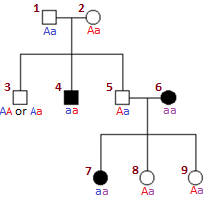
\includegraphics[width=.8\linewidth]{Figures/Picture2_recessive.png}
    \caption{Disorder is recessive}
\end{wrapfigure}
\par\noindent\textbf{B)\;\;\,} If the disorder allele was dominant, at-least one of $1$ or $2$ should have also had the disorder, as $4$ inherited it from them. Therefore, the disorder allele must be \textbf{recessive}. So $4,6$ and $7$ are \texttt{aa}. As $4$, and $7$ are \texttt{aa}, they have to get one \texttt{a} each from $1,2$ and $5,6$ respectively. Therefore $1,2$ and $5$ are \texttt{Aa}. As $6$ is \texttt{aa}, $8$ and $9$ are \texttt{Aa} (and not \texttt{AA}). We do not reach any inconsistency if the disorder is recessive.
\begin{align*}
    \textbf{Therefore the disorder has}\\
    \textbf{to be recessive.\hspace{1cm}}
\end{align*}\\\\\\

 

\end{document}